 \documentclass[10pt,a4paper]{article}
\usepackage{geometry}
 \geometry{
 a4paper,
 total={170mm,257mm},
 left=20mm,
 top=20mm,
 }


\usepackage[utf8]{inputenc}
\usepackage[spanish]{babel}
\usepackage{graphicx}
\usepackage{wrapfig}
\usepackage{amssymb, amsmath, siunitx}
\usepackage{tikz}
\usepackage{enumitem}
\usepackage{svg}
\usepackage{tcolorbox}
\usepackage{pdfpages}
\usepackage{mathtools}

\title{Flujo en conductos}
\author{Antonio Escámez Álvarez}
\date{Mayo 2021}


\setlength{\parindent}{0cm}

\begin{document}

\maketitle
\newpage
\tableofcontents
\newpage

Este tipo de problemas se resuelven partiendo de la ecuación de Bernoulli a la que le añadimos pérdidas.
\\

La ecuación de Bernoulli (despreciando pérdidas) indica que la enérgia entre 2 puntos permanece constante.
\\
Esto se expresa en la siguiente ecuación:
$$
\underbrace{\vphantom{\frac{}{}} P}_{\text{Término de presión}} + \underbrace{\frac{1}{2} \cdot \rho \cdot V^2}_{\text{Energía cinética}} + \underbrace{\vphantom{\frac{}{}}  \rho g z}_{\text{Energía Potencial}} = \text{Constante}
$$

Si igualamos Bernoulli en 2 puntos obtenemos la siguiente expresión:
$$
P_1 + \frac{1}{2} \cdot \rho \cdot V_{1}^2 + \rho g z = P_2 + \frac{1}{2} \cdot \rho \cdot V_{2}^2 + \rho g z 
$$

Si a esta ecuación le añadimos las pérdidas (primarias y secundarias que se explican a continuación) obtenemos la siguiente ecuación:

$$
P_1 + \frac{1}{2} \cdot \rho \cdot V_{1}^2 + \rho g z = P_2 + \frac{1}{2} \cdot \rho \cdot V_{2}^2 + \rho g z +  \frac{1}{2} \cdot \rho \cdot V_{m}^2 \cdot \left(\underbrace{\lambda \cdot \frac{L}{D}}_{\text Primarias} + \underbrace{\sum k}_{\text Secundarias} \right)
$$

\begin{center}
    \begin{tcolorbox}[colback=yellow!40!white, colframe=red!50!black,title=Ecuación de flujo en conductos]
    $$
        P_1 + \frac{1}{2} \cdot \rho \cdot V_{1}^2 + \rho g z = P_2 + \frac{1}{2} \cdot \rho \cdot V_{2}^2 + \rho g z +  \frac{1}{2} \cdot \rho \cdot V_{m}^2 \cdot \left(\lambda \cdot \frac{L}{D} + \sum k \right)
    $$
    \end{tcolorbox}
\end{center}

\newpage
\section{Lambda}
Lambda se obtiene en el diagrama de Moody, como podemos ver, Lambda es una función que depende de la rugosidad relativa ($\frac{\epsilon}{D}$) y del número de Reynolds (Re)
$$
\lambda = \lambda \left(\frac{\epsilon}{D},Re \right)
$$
En el caso de que no conozcamos $V_m$ y que no podamos calcularlo como $\frac{Q}{A}$, tenemos que suponer un valor de Reynolds elevado e iterar.
\\

Para iterar cogemos el valor de $\lambda$ directamente con la rugosidad relativa, con ese valor de $\lambda$ sustituimos en la ecuación que tengamos que resolver, con ese resultado de $V_m$ recalculamos Reynolds y con el diagrama de Moody volvemos a sacar un nuevo valor de $\lambda$ y procedemos así tantas veces como sea necesario hasta que el valor de $\lambda$ sea constante.

\section{Reynolds}
Por otro lado Reynolds se calcula como:
$$
Re = \frac{\rho \cdot V_m \cdot D}{\mu} = \frac{1}{10^{-6}} \cdot V_m \cdot D = \frac{V_m \cdot D}{10^{-6}}
$$

\begin{center}
    \begin{tcolorbox}[colback=yellow!40!white, colframe=red!50!black, width=5cm,title=Ecuación de Reynolds]
    $$
        Re =  \frac{V_m \cdot D}{10^{-6}}
    $$
    \end{tcolorbox}
\end{center}

\section{Caudal}
El caudal se calcula como:

\begin{center}
    \begin{tcolorbox}[colback=yellow!40!white, colframe=red!50!black, width=5cm,title=Caudal]
    $$
        Q = V \cdot A \,\,\, \left[ \frac{m^3}{s} \right]
    $$
    \end{tcolorbox}
\end{center}

\section{Potencia de una bomba}
El trabajo de una bomba se calcula como:
\begin{center}
    \begin{tcolorbox}[colback=yellow!40!white, colframe=red!50!black, width=5cm,title=Potencia de una bomba]
    $$
        \dot{W} = Q \cdot \bigtriangleup P \,\,\, [W]
    $$
    \end{tcolorbox}
\end{center}

\newpage
\section{Presión a la entrada de un depósito}
Cuando trabajamos con un depósito como el siguiente:
\begin{center}
    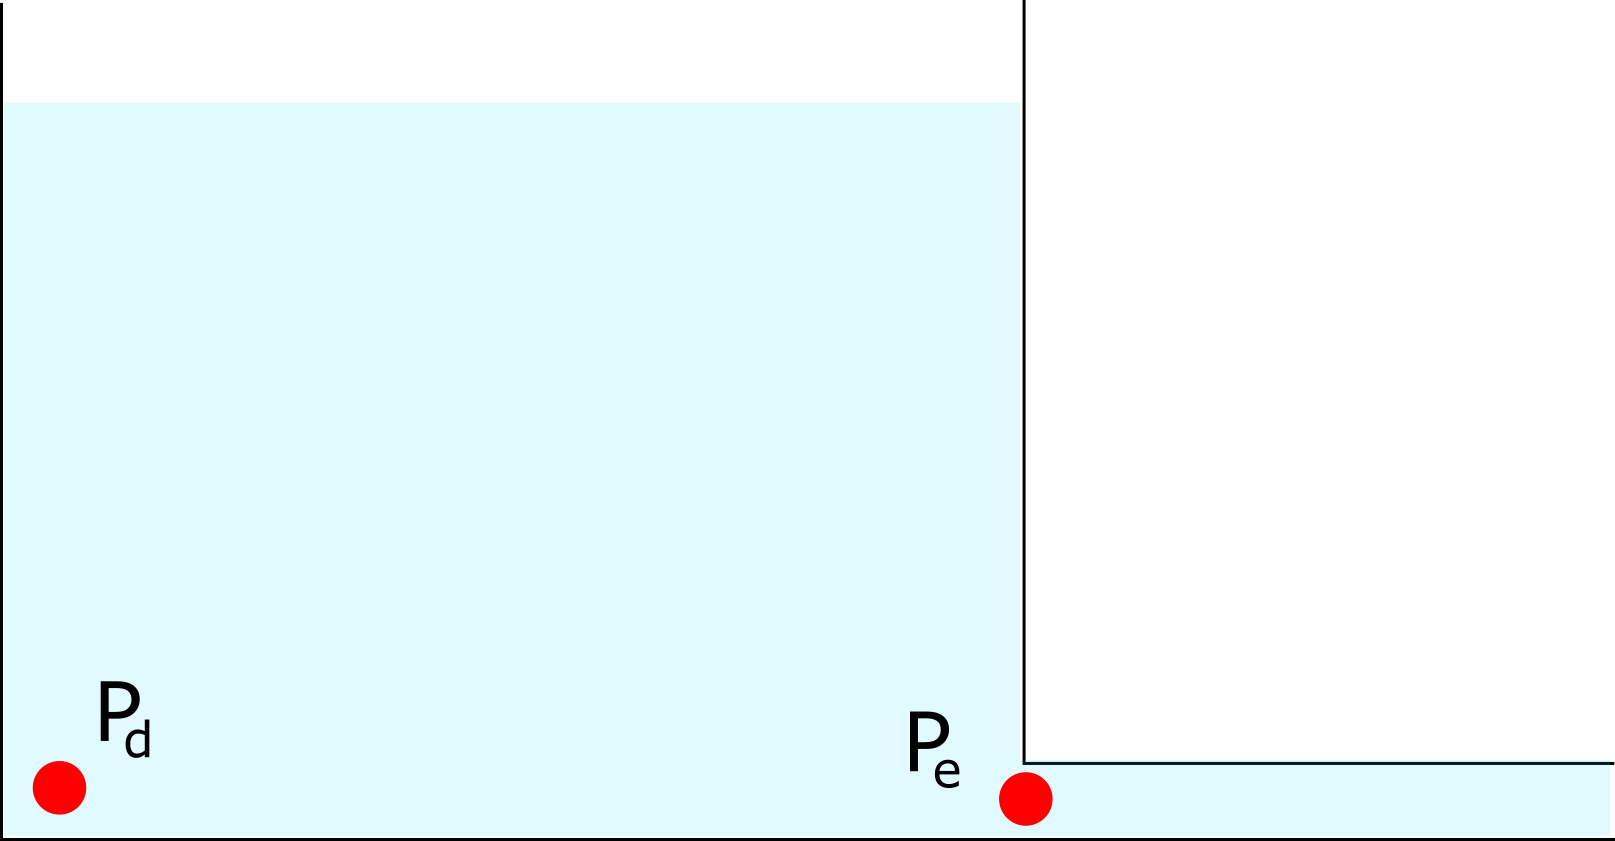
\includegraphics[scale = 0.6]{Deposito.png}
\end{center}

Tenemos que tener en cuenta que la presión reducida en la entrada es la presión del fondo del depósito ($P_d$) menos la energía que contiene.
$$
P_e = P_d - \frac{1}{2} \cdot \rho \cdot V_m^2 \cdot \left( 1 + K_e \right)
$$

Donde $P_d$ se puede calcular como:
$$
P_d = P_a + \rho g z
$$

En general obtenemos que:

\begin{center}
    \begin{tcolorbox}[colback=yellow!40!white, colframe=red!50!black, width=9cm,title=Presión a la entrada de un depósito]
    $$
        P_e = P_a + \rho g z - \frac{1}{2} \cdot \rho \cdot V_m^2 \cdot \left( 1 + K_e \right)
    $$
    \end{tcolorbox}
\end{center}

\section{Sustituir $V_m^2$ en función de Q}
$$
Q = V_m \cdot A \xrightarrow{\text{Sustituyo A}} Q = V_m \cdot \frac{\pi \cdot D^2}{4} \xrightarrow{\text{Despejo $V_m$}} 
$$

$$
V_m = \frac{4 \cdot Q}{\pi \cdot D^2} 
$$

Si tengo que sustituir $V_m^2$:
$$
V_m^2 = \frac{16 \cdot Q^2}{\pi^2 \cdot D^4}
$$

Se suele sustituir en la fórmula:
$$
\frac{1}{2} \cdot \rho \cdot V_m^2
$$

Obteniendo:
\begin{center}
    \begin{tcolorbox}[colback=yellow!40!white, colframe=red!50!black, width=9cm,title=Sustituir $V_m^2$ por Q]
    $$
        \frac{1}{2} \cdot \rho \cdot V_m^2 = \frac{8 \cdot \rho \cdot Q^2}{\pi^2 \cdot D^4}
    $$
    \end{tcolorbox}
\end{center}

\newpage
\section{Expansión y contracción brusca}
La perdida de carga en una expansión brusca podemos calcularla como:
\begin{center}
    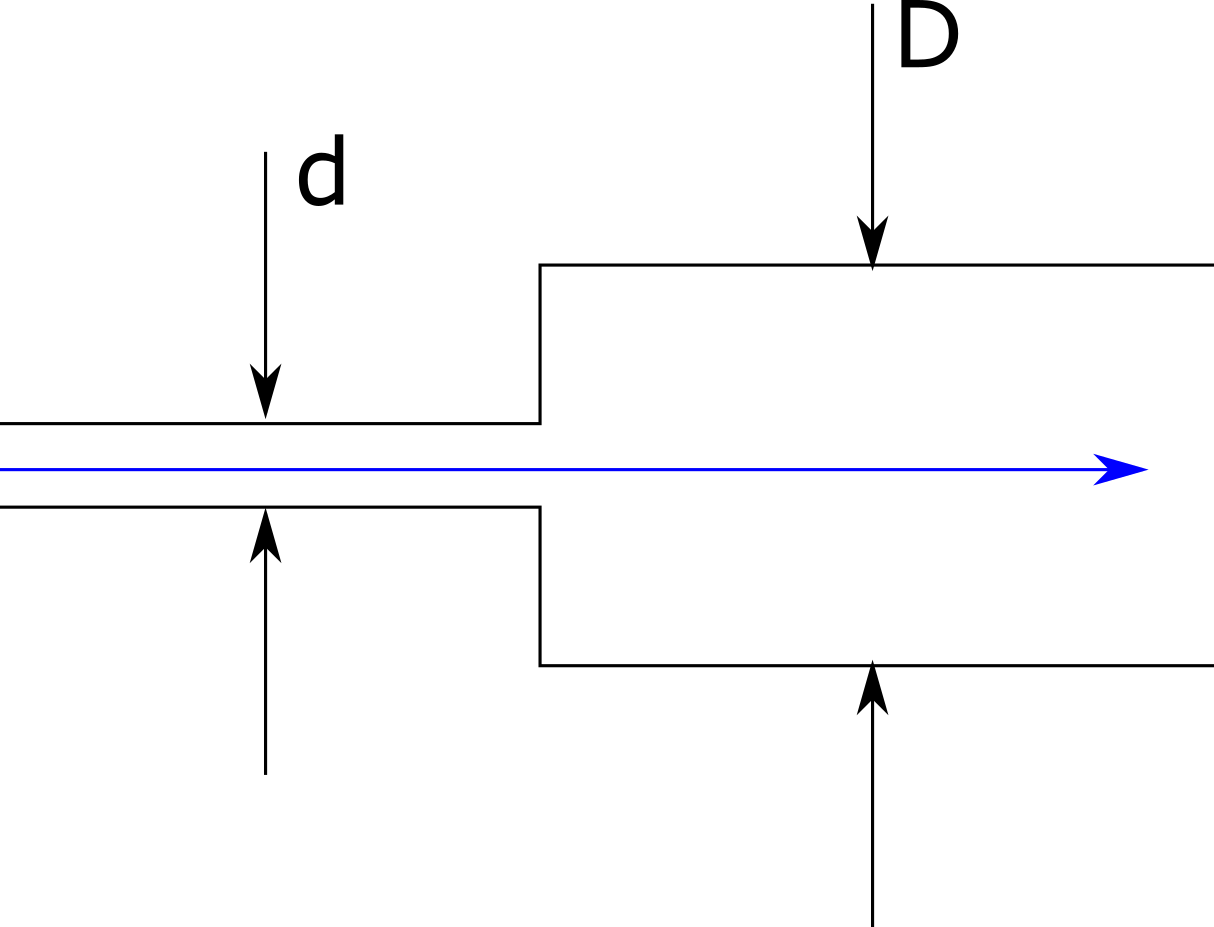
\includegraphics[scale = 0.5]{Expansion Brusca.png}
    \begin{tcolorbox}[colback=yellow!40!white, colframe=red!50!black, width=9cm,title=Expansión Brusca]
    $$
        K_{eb} = \left[ 1 - \left( \frac{d}{D} \right)^2 \right]^2
    $$
    \end{tcolorbox}
\end{center}

La perdida de carga en una contracción brusca podemos calcularla como:
\begin{center}
    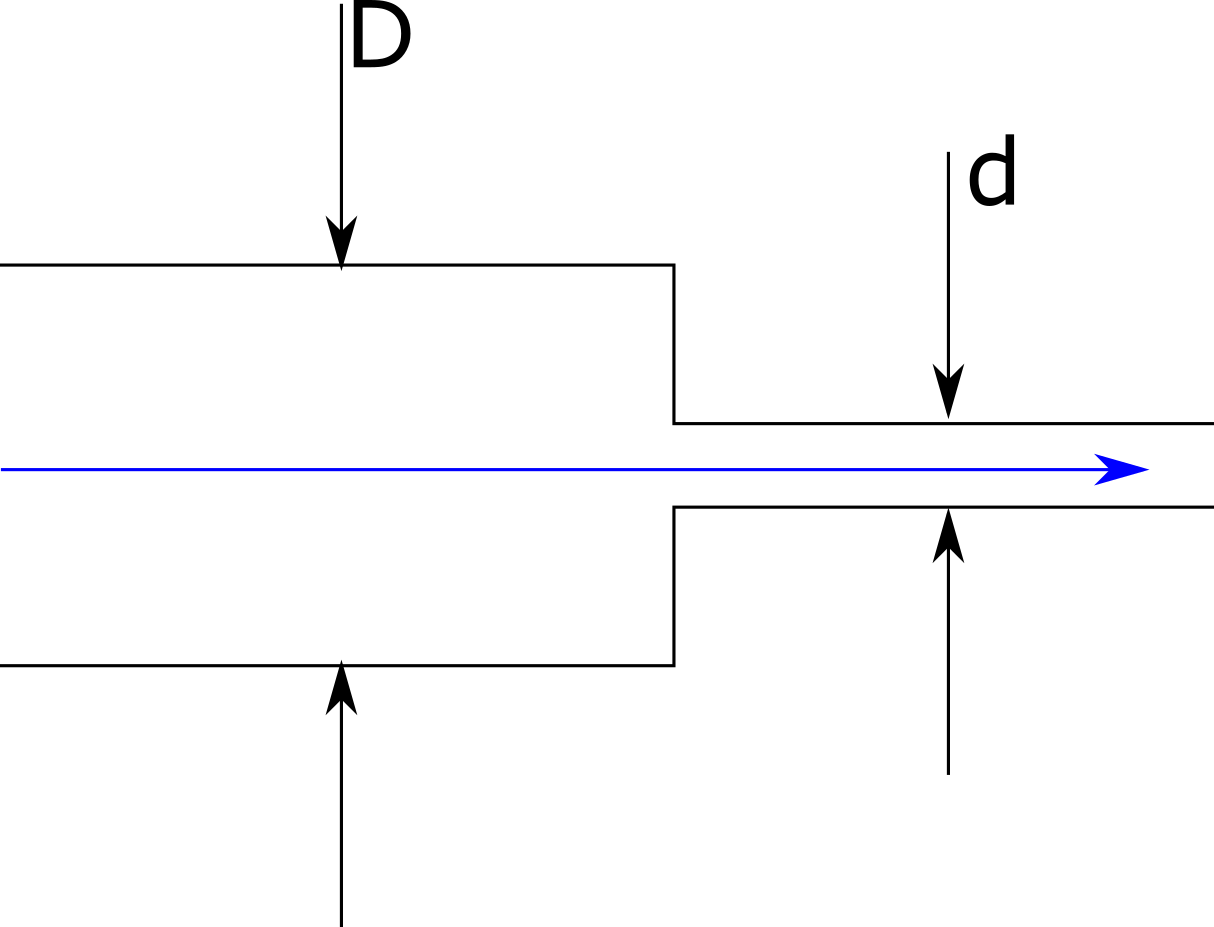
\includegraphics[scale = 0.5]{Contraccion Brusca.png}
    \begin{tcolorbox}[colback=yellow!40!white, colframe=red!50!black, width=9cm,title=Contracción Brusca]
    $$
        K_{cb} = 0.5 \cdot \left[ 1 - \left( \frac{d}{D} \right)^2 \right]
    $$
    \end{tcolorbox}
\end{center}

Estas pérdidas se referencian siempre al $\lambda$ mas pequeño, es decir:
\\

Si tengo tres tamaños de tubería $D_1, D_2, D_3$ que son mas grandes respectivamente, si tengo una expansión/contracción de $D_1$ a $D_2$ esta pérdida ira acompañando a $D_1$.
\\
Si tengo una expansión/contracción de $D_2$ a $D_3$ esta pérdida ira acompañando a $D_2$.
\\
Como podemos observar $D_3$ no tiene referenciada pérdidas secundarias por expansión/contracción ya que no desemboca en otra tubería mas grande.
\\

Diciéndolo de otro modo, la $K_e$ se pone si la tubería que estoy estudiando es mas pequeña que la tubería que tiene la expansión/contracción.

\newpage
\section{Símil hidráulico - eléctrico}

Cuando tenemos el siguiente esquema:
\begin{center}
    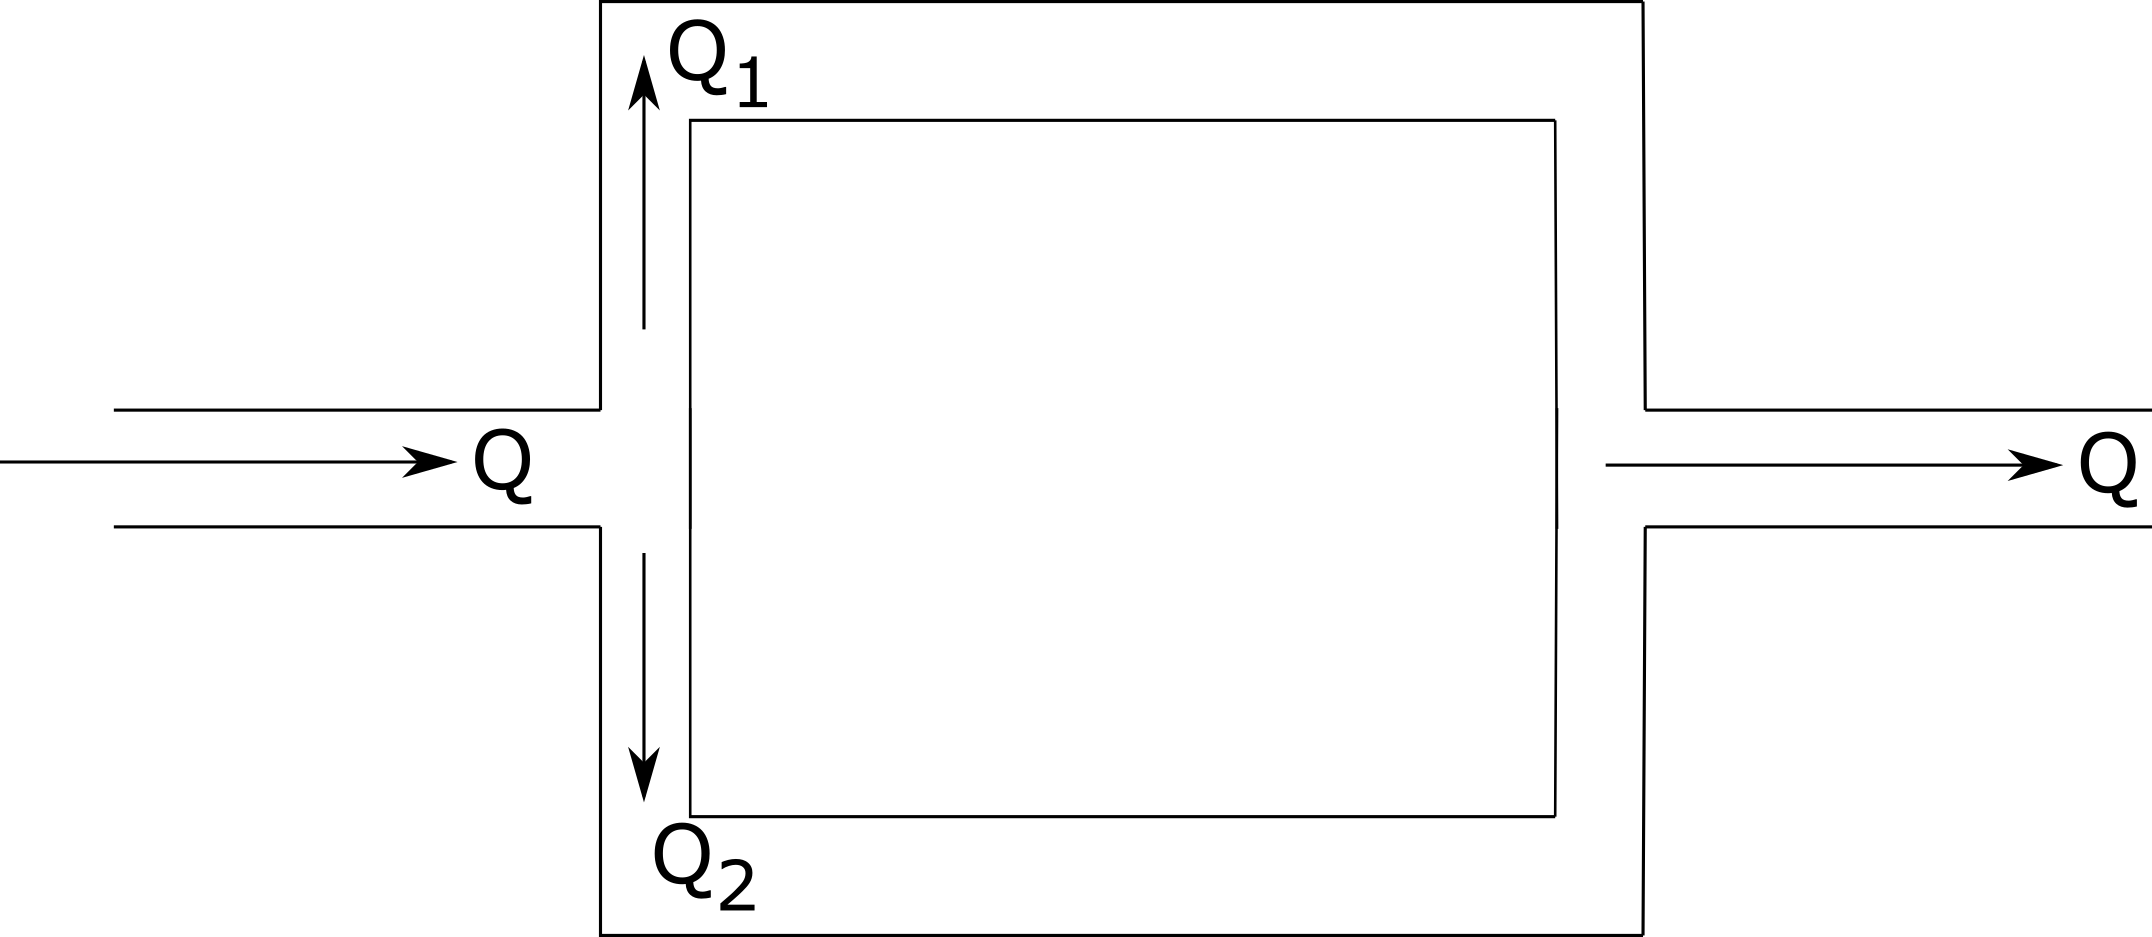
\includegraphics[scale = 0.5]{Division.png}
\end{center}
Podemos verlo como un circuito eléctrico haciendo la siguiente comparación:
\begin{center}
\begin{tabular}{ |c|c| } 
 \hline
 Q & A \\ 
 \hline
 $\bigtriangleup$ P & $\bigtriangleup$ V \\ 
 \hline
 K & R \\ 
 \hline
\end{tabular}
\end{center}
Podemos deducir que:
$$
\bigtriangleup P_1 = \bigtriangleup P_2
$$

\section{Ejemplo}
Tenemos una tubería con 3 secciones $D, D_1, D2$ y con varios elementos como codos valvulas etc.

A la hora de plantear la ecuación general es importante recordar que vamos a disponer de 3 $\lambda$ ya que tenemos 3 secciones diferentes y por tanto la velocidad del caudal va a variar y por ende el Reynolds.
\begin{center}
    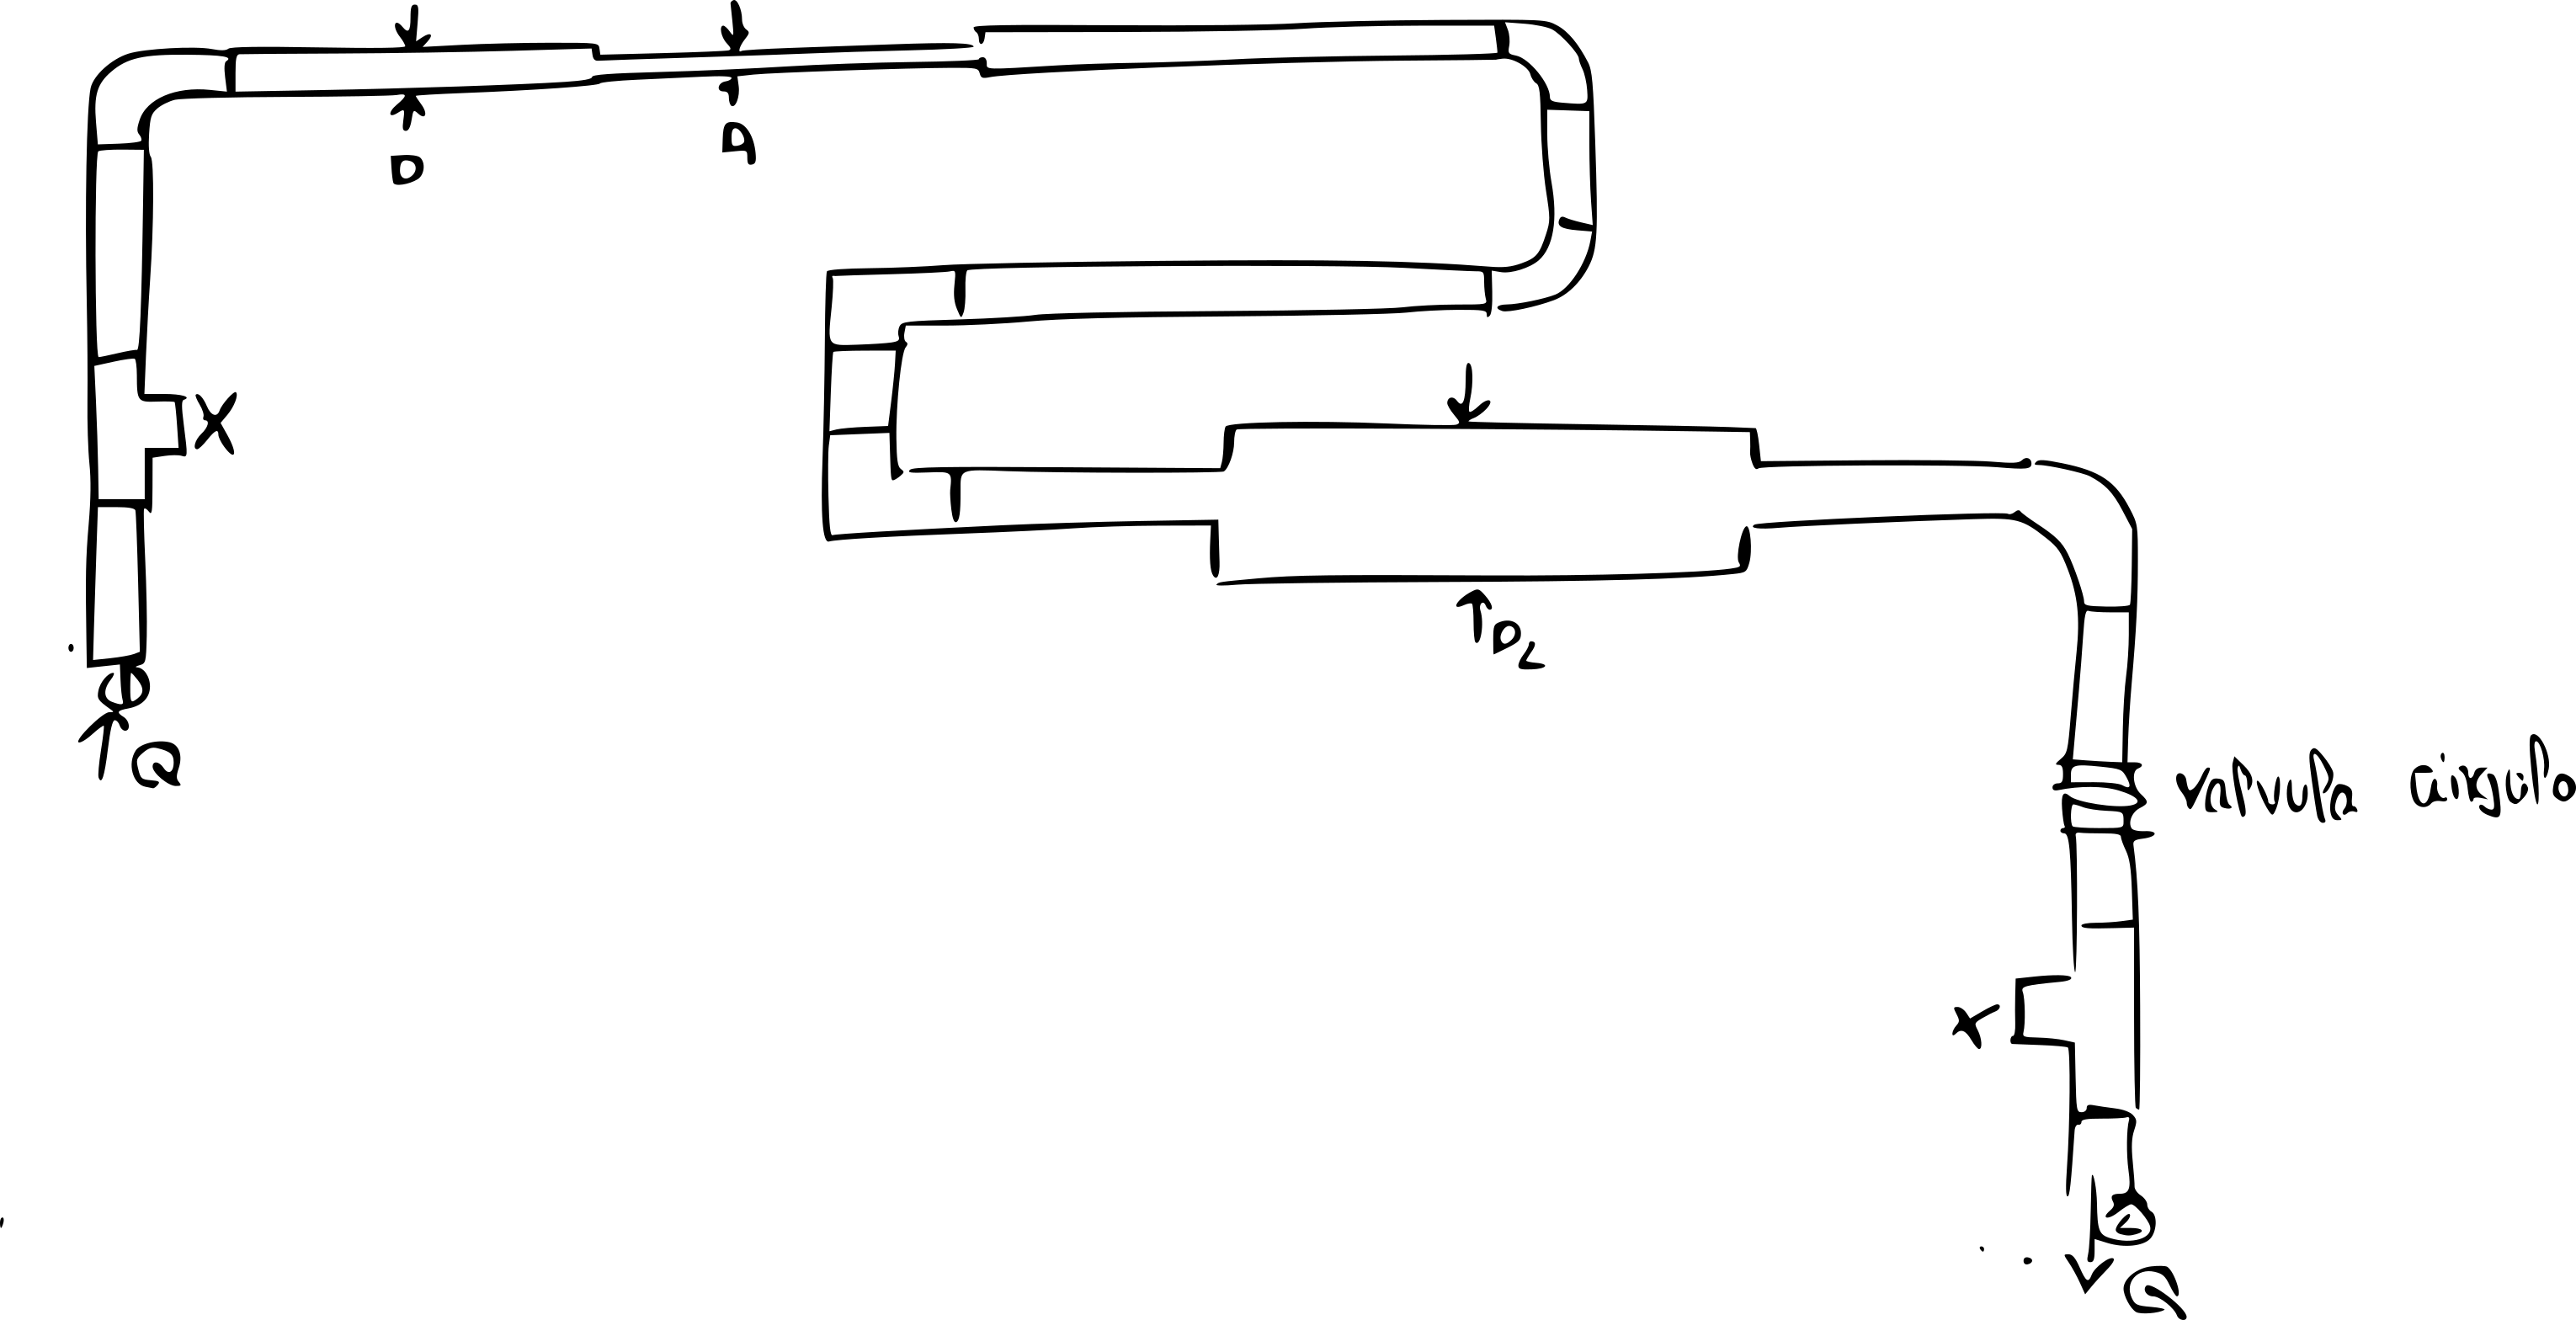
\includegraphics[scale = 0.6]{Ejemplo Vector.png}
\end{center}
Vamos a plantear la ecuación entre la entrada y la salida. Una vez vemos que las velocidades en esos dos puntos son iguales y que el potencial (z = 0) obtenemos la siguiente expresión:
$$
P_1 - P_2 = \underbrace{\frac{1}{2} \cdot \rho \cdot V_m^2 \left(\overbrace{\lambda \frac{L}{D}}^{\text{Primarias}} + \overbrace{2\cdot K_{\text{Te}} + 4\cdot K_{\text{curva suave}} + 2\cdot K_{\text{codo}} + K_{\text{valvula angulo}} + K_{\text{eb D$\xrightarrow{}{}D_2$}} + K_{\text{cb $D_2 \xrightarrow{}$D}}}^{\text{Secundarias}}\right)}_{\text{Sección D}} + 
$$
$$
+ \underbrace{\frac{1}{2} \cdot \rho \cdot V_{m1}^2 \left(\lambda_1 \frac{L_1}{D_1} + K_{eb D_1 \xrightarrow{} D} + K_{ec D \xrightarrow{}D_1} \right)}_{\text{Sección $D_1$}} + \underbrace{\frac{1}{2} \cdot \rho \cdot V_{m2}^2 \left(\lambda_2 \frac{L_2}{D_2} \right)}_{\text{Sección $D_2$}}
$$

\newpage
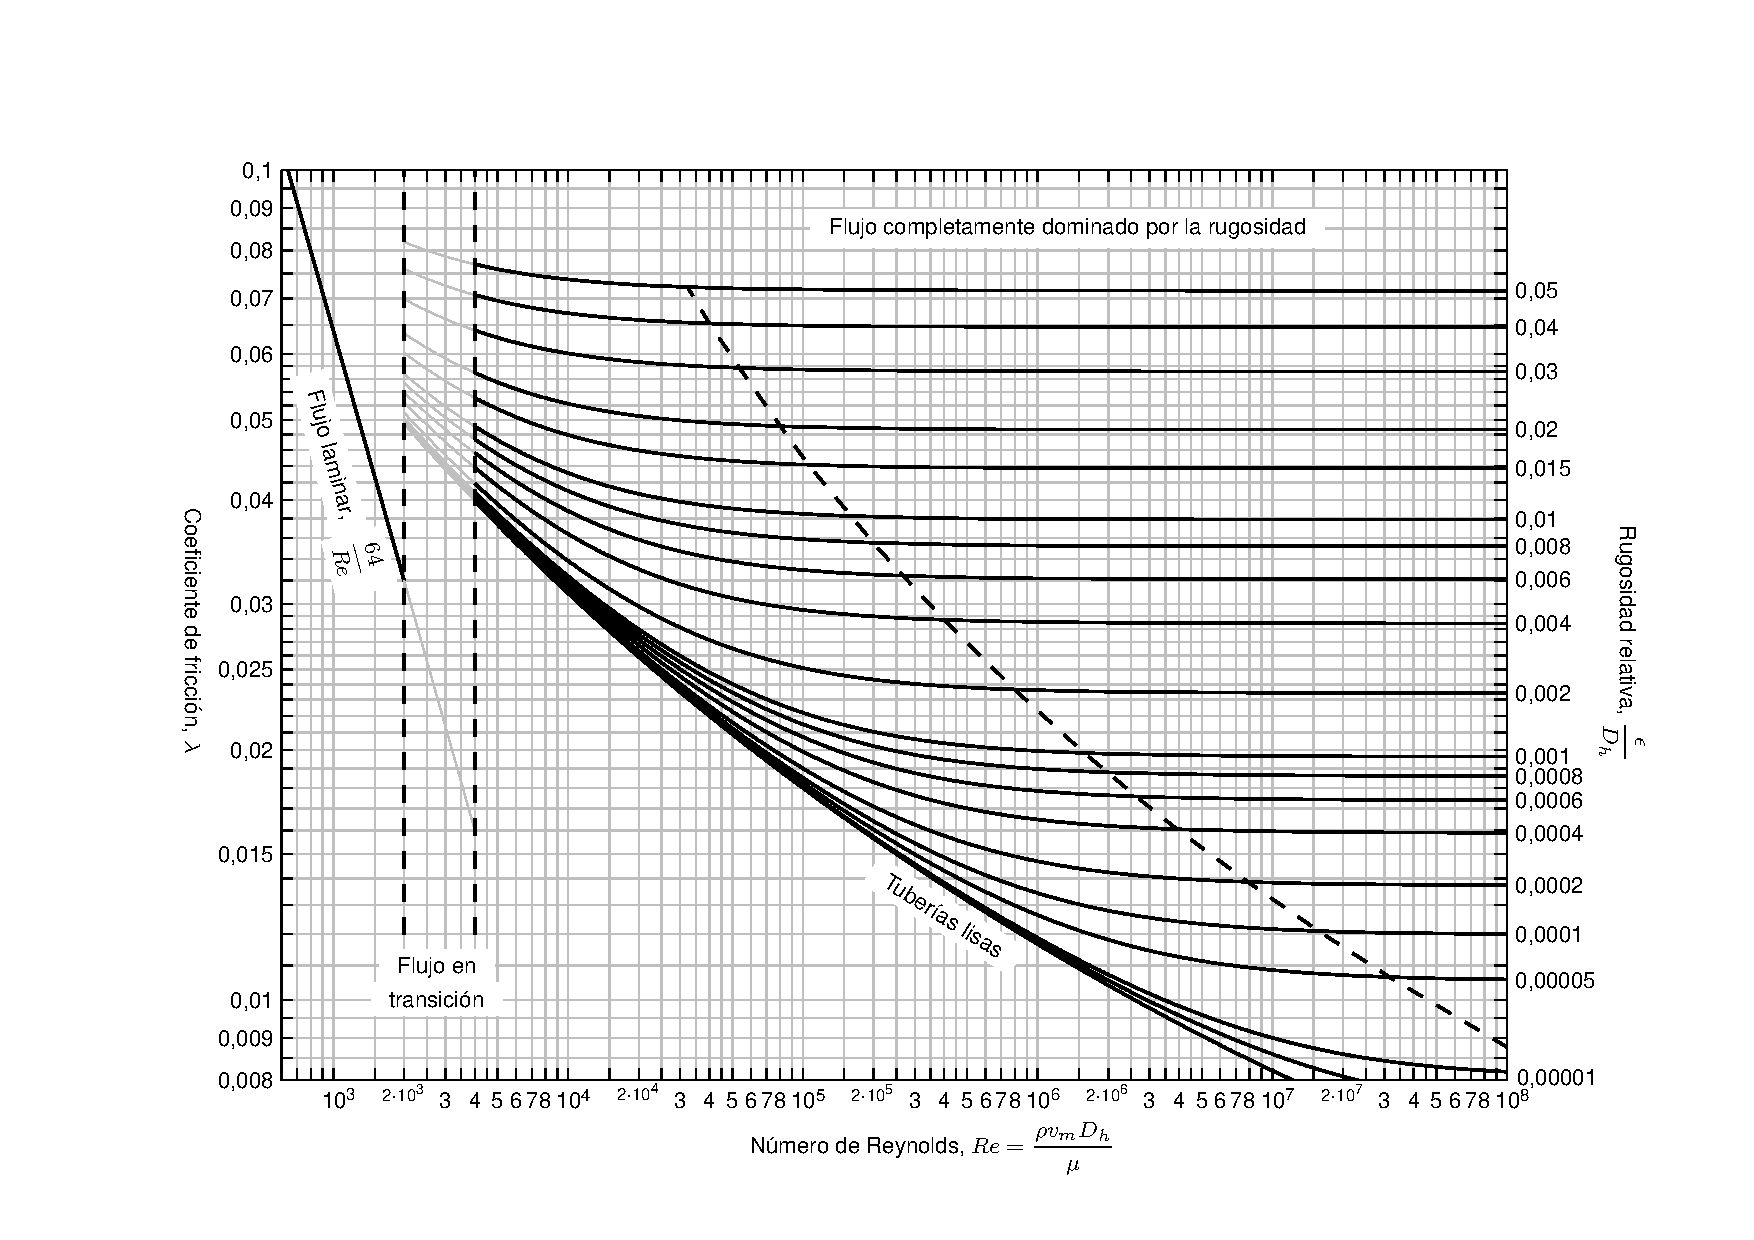
\includepdf[angle = 90, scale = 0.9,pagecommand=\section{Diagrama de Moody}]{Diagrama de Moody.pdf}

\end{document}
